%% Optimask Data Structure
%% Created: 2017-08-23; Updated: 2017-08-23;
%% by Henghua DENG, hdeng@optixera.com

\resetdatestamp %Date Stamp--Only use when custom package datestamp.sty is used.

%\part{Optimask Layout Design} \label{PartMaskDesign}
%本部分介绍Optimask版图设计软件基本框架,具体功能实现,主要界面,命令行及编程输入等等。

\chapter{Optimask Data Structure} \label{ChMaskDataStruct}
%======================================================================
%Heading Settings:
\markboth{Chapter~\thechapter.~Data~Structure}{} %\leftmark calls #1 parameter
%\markright{ } % new right header. Only used for two-side documents.

\pagestyle{fancy}
\fancyhead[RO,RE]{}
\fancyhead[LE]{\MakeUppercase{\leftmark}}
\fancyhead[LO]{\MakeUppercase{\rightmark}}
\fancyfoot[C]{\thepage}
%%\fancyfoot[L]{\today}

Optimask版图设计的数据结构(Data Structure)是非常重要的基本构架。Optimask版图数据结构基于GDSII格式,但是做了重要扩展为自定义格式。当版图Tape-Out时,自定义格式可以转换为标准GDSII格式。

%======================================================================
\section{Optimask数据结构基本构架} \label{SectDataStruct}
%======================================================================
Optimask数据结构基本构架其实很简单,主要分为基本图元(Element)和构元引用(Reference)两类。

\begin{figure}[htb!p] %h--here, t--top, b--bottom, p--page;
	\centering
	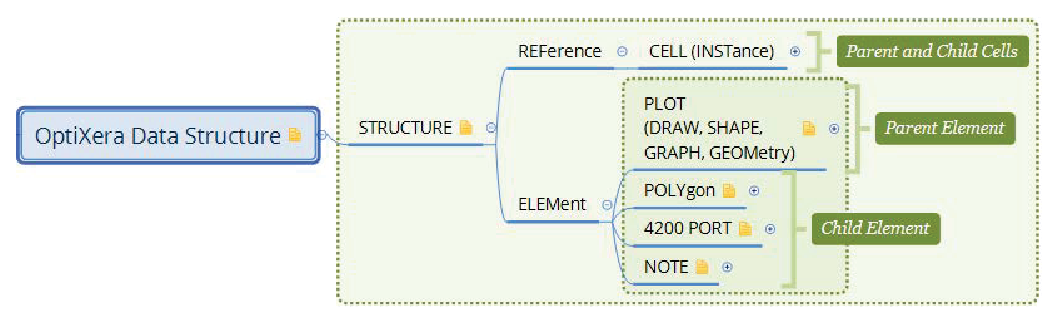
\includegraphics[width=4in]{./Layout/FigsData/Structure.eps}
	\caption{Optimask数据结构基本构架。}
	\label{FigDataStruct}
\end{figure}

%======================================================================
\section{Optimask基本图元(Element)数据结构} \label{SectDataElem}
%======================================================================
Optimask基本图元(Element)数据结构,包括绘制(Plot)、多边形(Polygon)、端口(Port)和标注(Note)。

基本图元(Element)是指所有尚没有组成构元结构的基本图形。GDSII格式主要包括矩形(Box), 多边形(Polygon), 线(Wire)等。其实所有的图形都可以转换为多边形(Polygon)。但是对于很多规则图形,直接存储为多边形比较占用空间。比如圆形,不管用多少个点近似为多边形,都不如直接存储圆心位置和半径大小准确和简洁。所以我们将基本图形稍微扩展出绘制(Plot)子结构。

基本图元(Element)之间的连接信息也经常需要用到。比如,对于光波导和微波波导等,经常需要确定光路和电磁波的路径。此时不同器件之间需要用端口(Port)来连接。

我们希望版图的理解和信息传递尽量有效,所以同时定义了标注(Note)来存储重要的设计信息。

\begin{figure}[htb!p] %h--here, t--top, b--bottom, p--page;
	\centering
	\subfigure[绘制(Plot)和多边形(Polygon)] {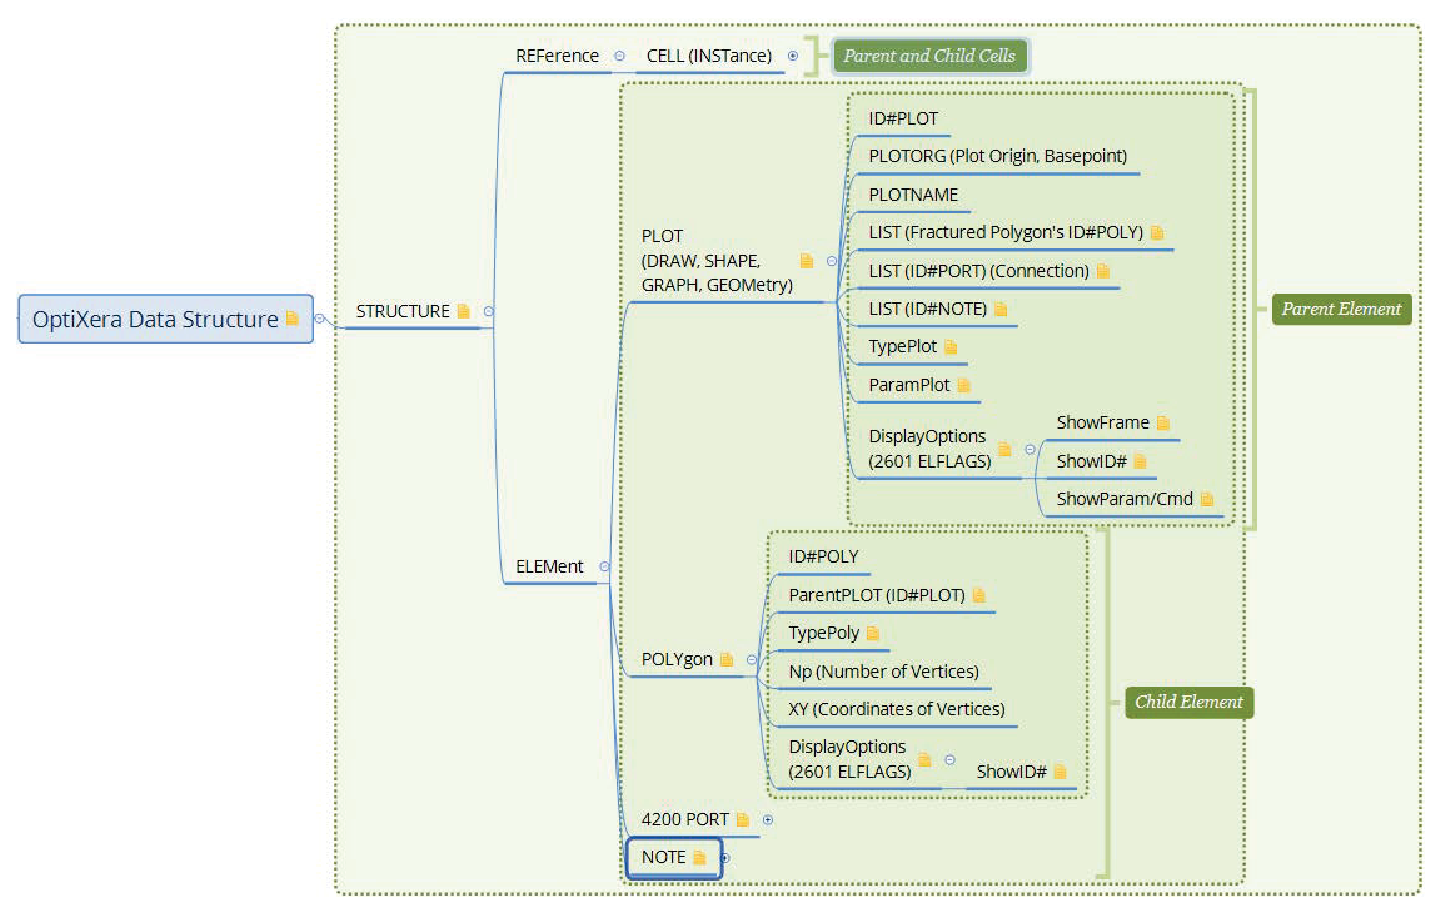
\includegraphics[width=3in]{./Layout/FigsData/ElemPlotPoly.eps}
		\label{FigDataElemPlotPoly}}
	\hfill
	\subfigure[端口(Port)和标注(Note)] {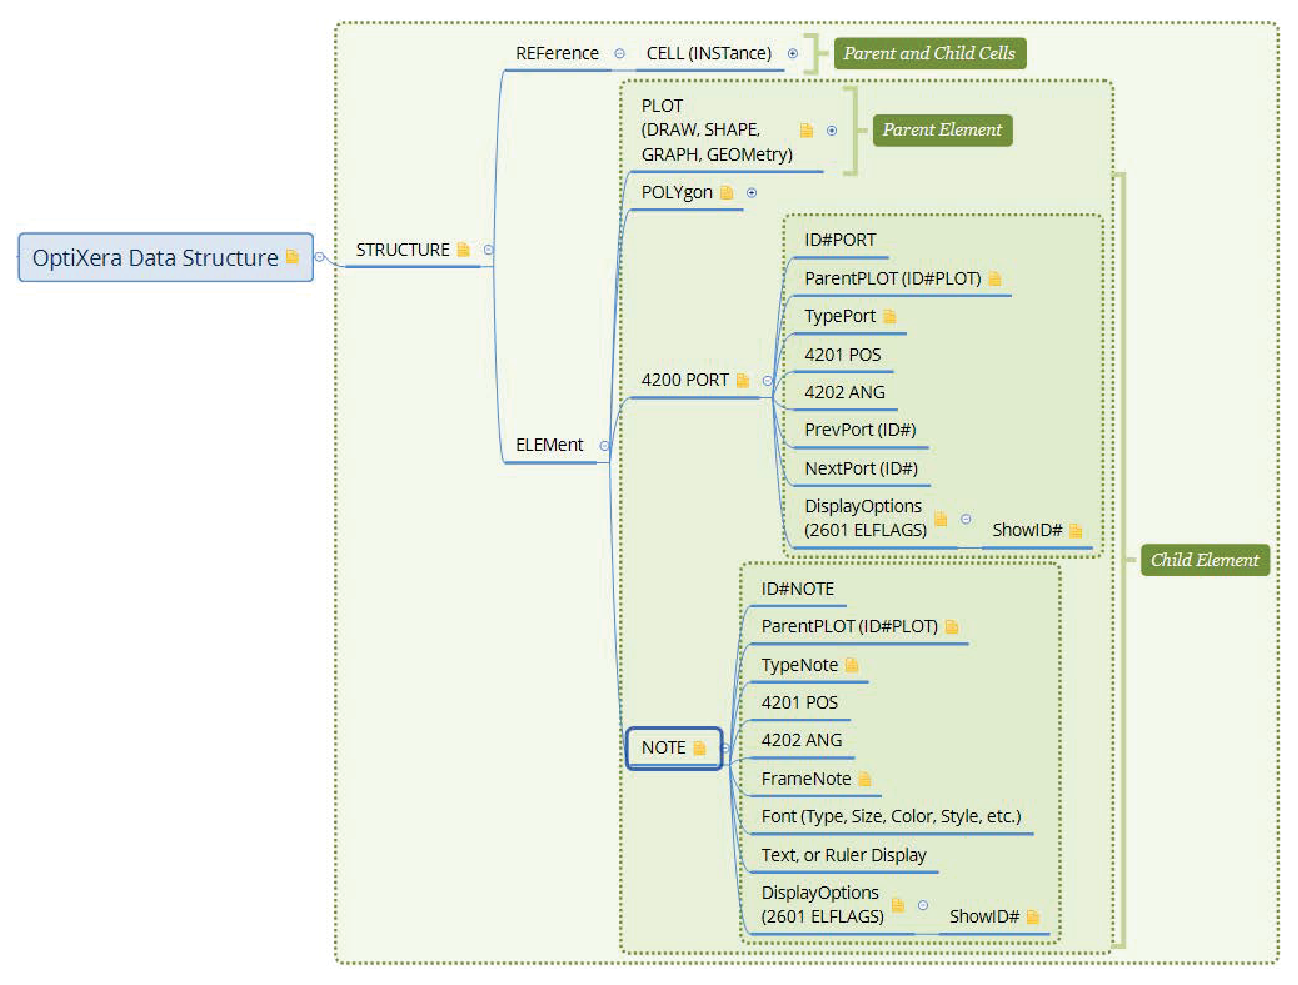
\includegraphics[width=3in]{./Layout/FigsData/ElemPortNote.eps}
		\label{FigDataElemPortNote}}
	\caption{Optimask基本图元(Element)数据结构,包括绘制、多边形、端口和注释。}
	\label{FigDataElem}
\end{figure}

\subsection{绘制(Plot)} \label{SectDataPlot} 
绘制(Plot)。

\subsection{多边形(Polygon)} \label{SectDataPoly} 
多边形(Polygon)。

\subsection{端口(Port)} \label{SectDataPort}
端口(Port)。

\subsection{标注(Note)} \label{SectDataNote} 
标注(Note)。

%======================================================================
\section{Optimask构元引用(Cell Reference)数据结构} \label{SectDataRef}
%======================================================================
Optimask构元引用(Cell Reference)数据结构。
\begin{figure}[htb!p] %h--here, t--top, b--bottom, p--page;
	\centering
	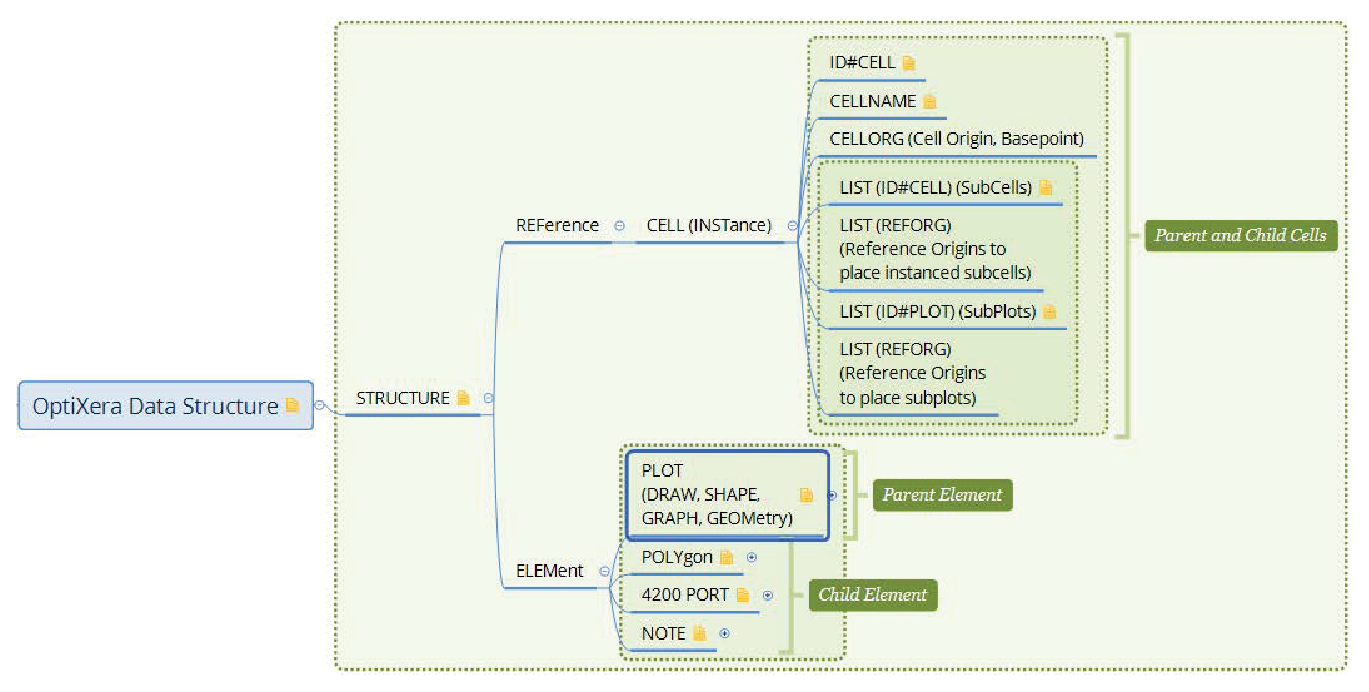
\includegraphics[width=4in]{./Layout/FigsData/RefCell.eps}
	\caption{Optimask构元引用(Cell Reference)数据结构。}
	\label{FigDataRef}
\end{figure}

%%\pagestyle{empty}
%%\cleardoublepage
%%to generates one blank page for the next chapter to be on an odd page
